\documentclass[PROP_AGutteridge_CS.tex]{subfiles}

\begin{document}

\chapter{Related Work}
Comparable systems will be reviewed and contrasted in order to provide context to the proposed project.

\section{GoPubMed: An Ontology-Driven Search Engine}
Developed by Michael Schroeder and colleagues at Dresden University, GoPubMed (\url{http://gopubmed.com/}) is a server and web interface that provides PubMed search results informed by the Gene Ontology database\cite{doms}. By extracting terms present in the Gene Ontology database from abstracts, GoPubMed has an improved vocabulary for genes and the gene products, enabling discovery of relevant papers that may be missed by the default PubMed search algorithm. The web interface also has additional functionality by providing shortcuts to 'Highly Related Concepts', authors and locations (Fig.1a), as well as visual representations of the data (Fig.1b) \\

\noindent Due to the aims of the project as described\cite{doms}, the applicability is largely limited to the field of Molecular Biology where genes and proteins are of primary interest. In the sidebar, both 'Highly Related Concepts' and 'All related Concepts' are drop-down menus providing keywords that are most prevalent in the citations retrieved by the search algorithm. This approach may be suitable for the proposed project, as it highlights research and publication trends. For this project I would suggest a narrowed vocabulary of related topics. The most common 'Highly Related Concepts' that appear on GoPubMed are often generic. For example, the top three 'Highly Related Concepts' resulting from the search term 'pancreatic cancer' are: Middle Aged, Survival, and Pancreatectomy\footnote{Query ran 07/04/15.}, arguably only the last of which could be of conducive to a user's search. Additional filters are also provided as part of the interface, allowing the user to specify, for example, that only papers authored in the United Kingdom should be shown. A map of authors is generated from all results pages (Fig.1b), the static property of which precludes direct user interaction. \newpage

\begin{figure}[h!]
	\begin{subfigure}{1\textwidth}
		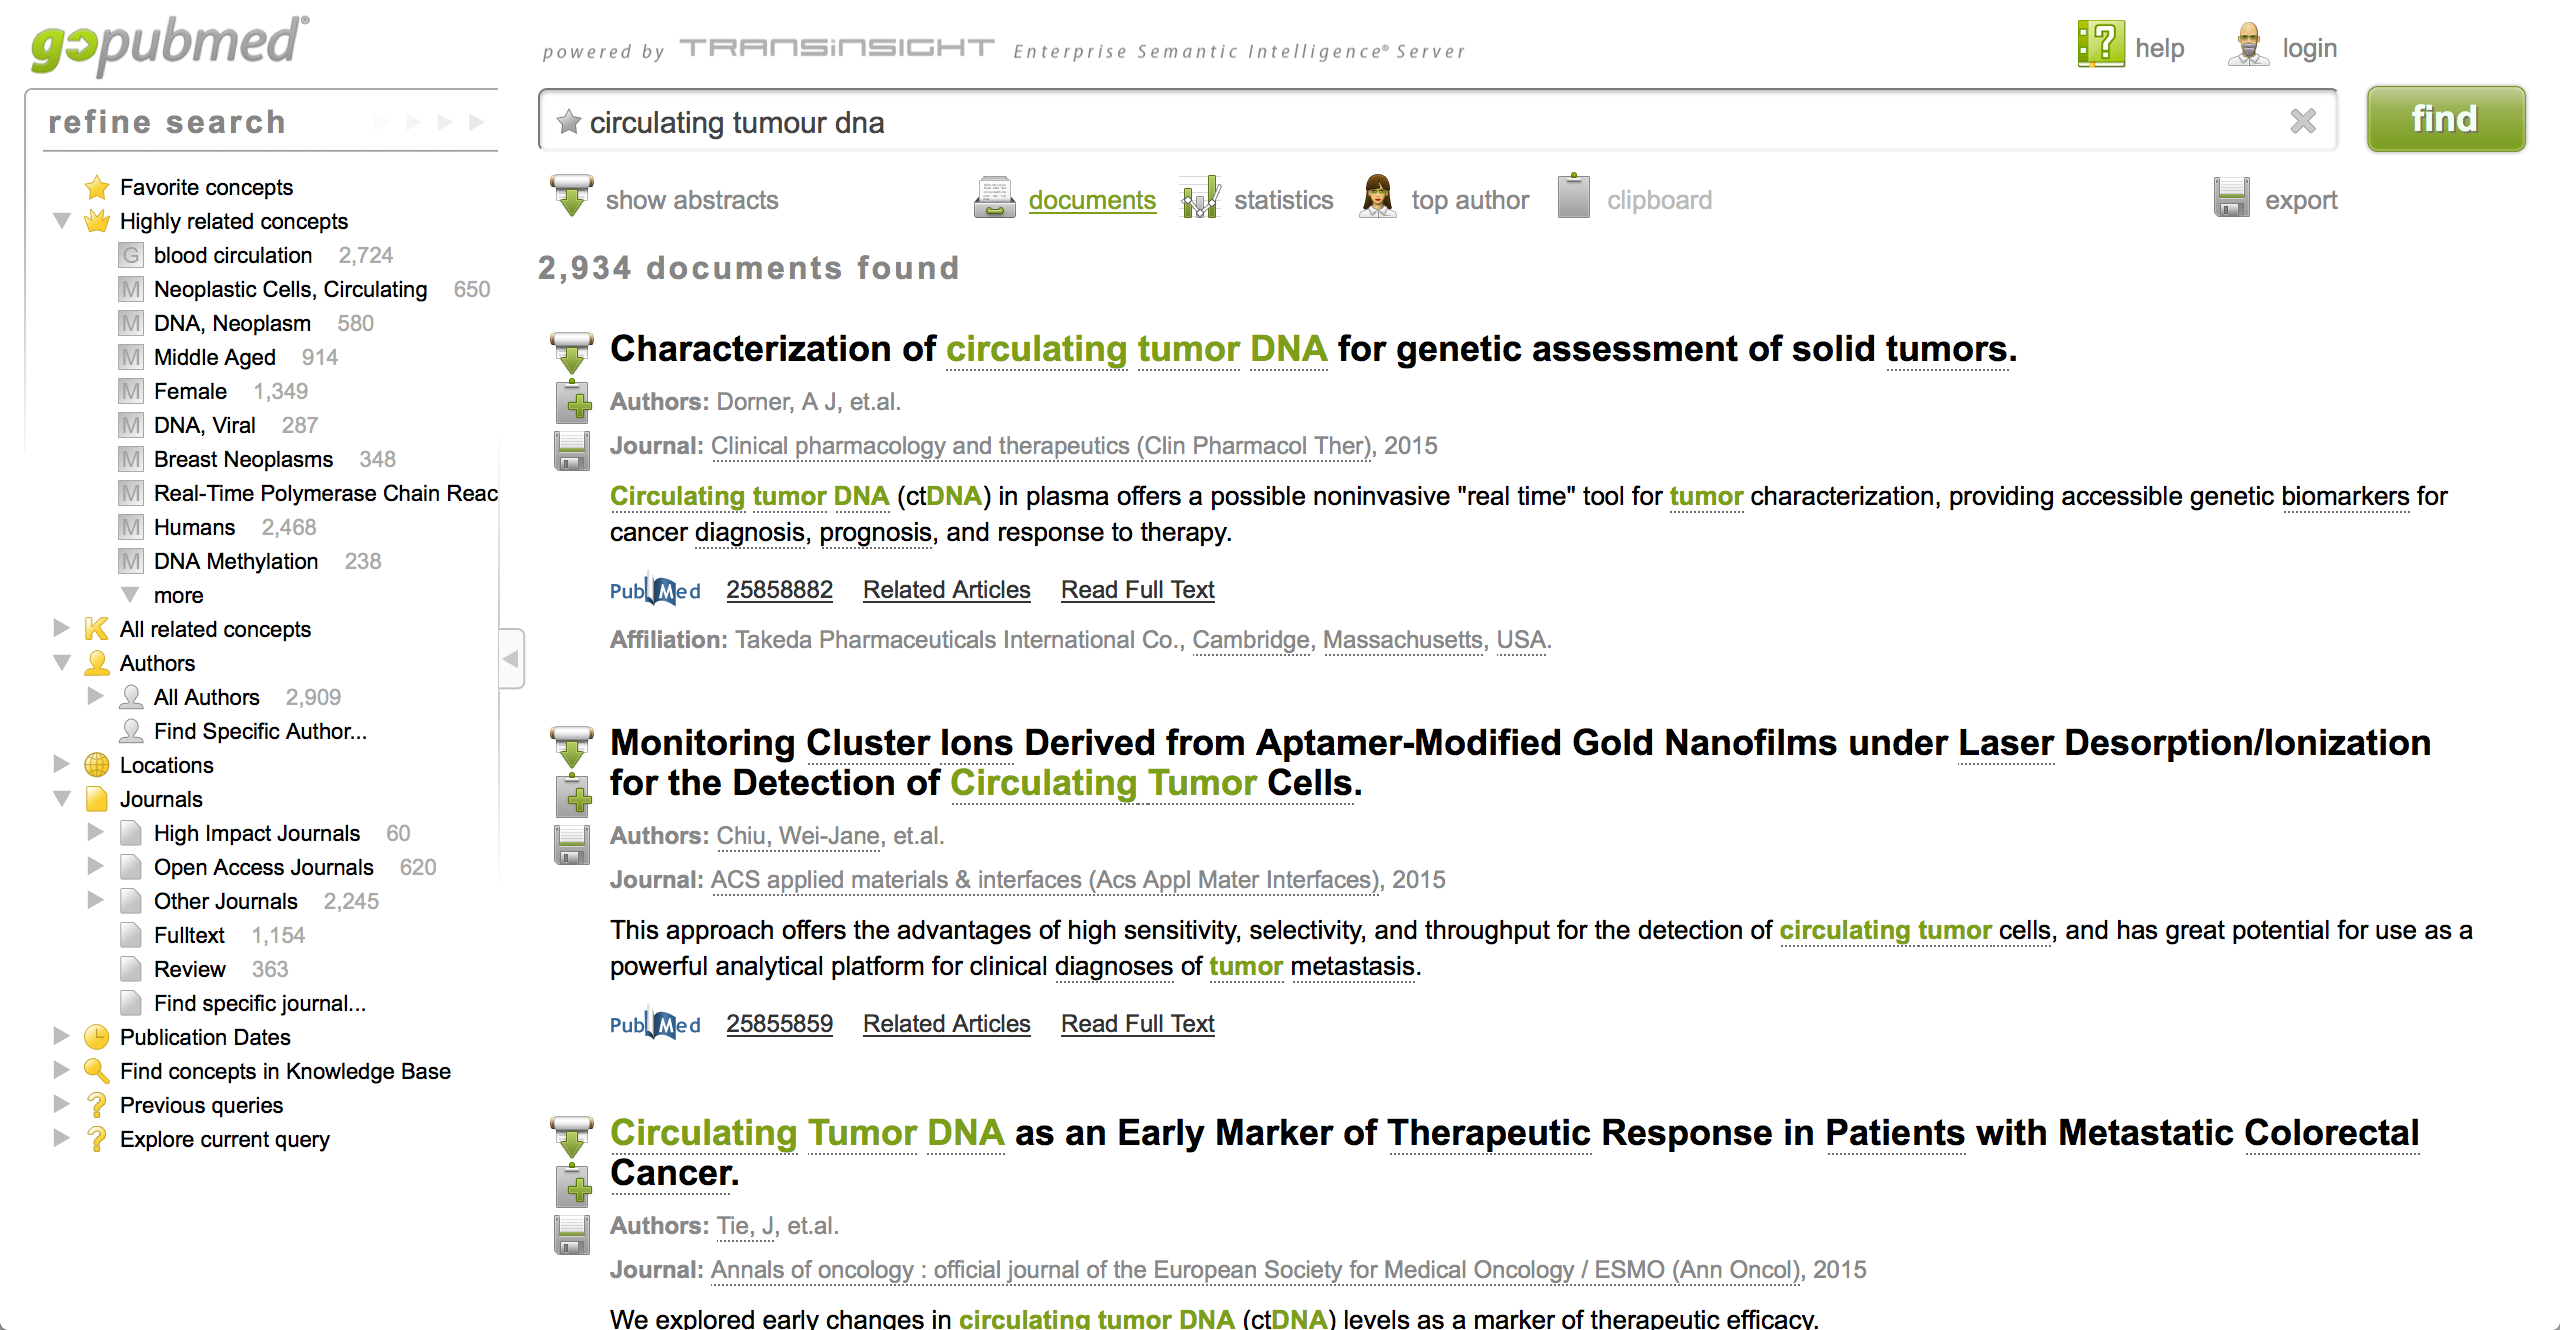
\includegraphics[width=\textwidth]{../lib/images/GPM1}
		\label{fig:GPM1}
		\subcaption{Documents view: screen after a search term has been entered. The main component of the page is the list of relevant documents, ordered by latest publication date. Additional filters are available in the sidebar to the left.}
	\end{subfigure}\\
	\par\bigskip
	\begin{subfigure}{1\textwidth}
		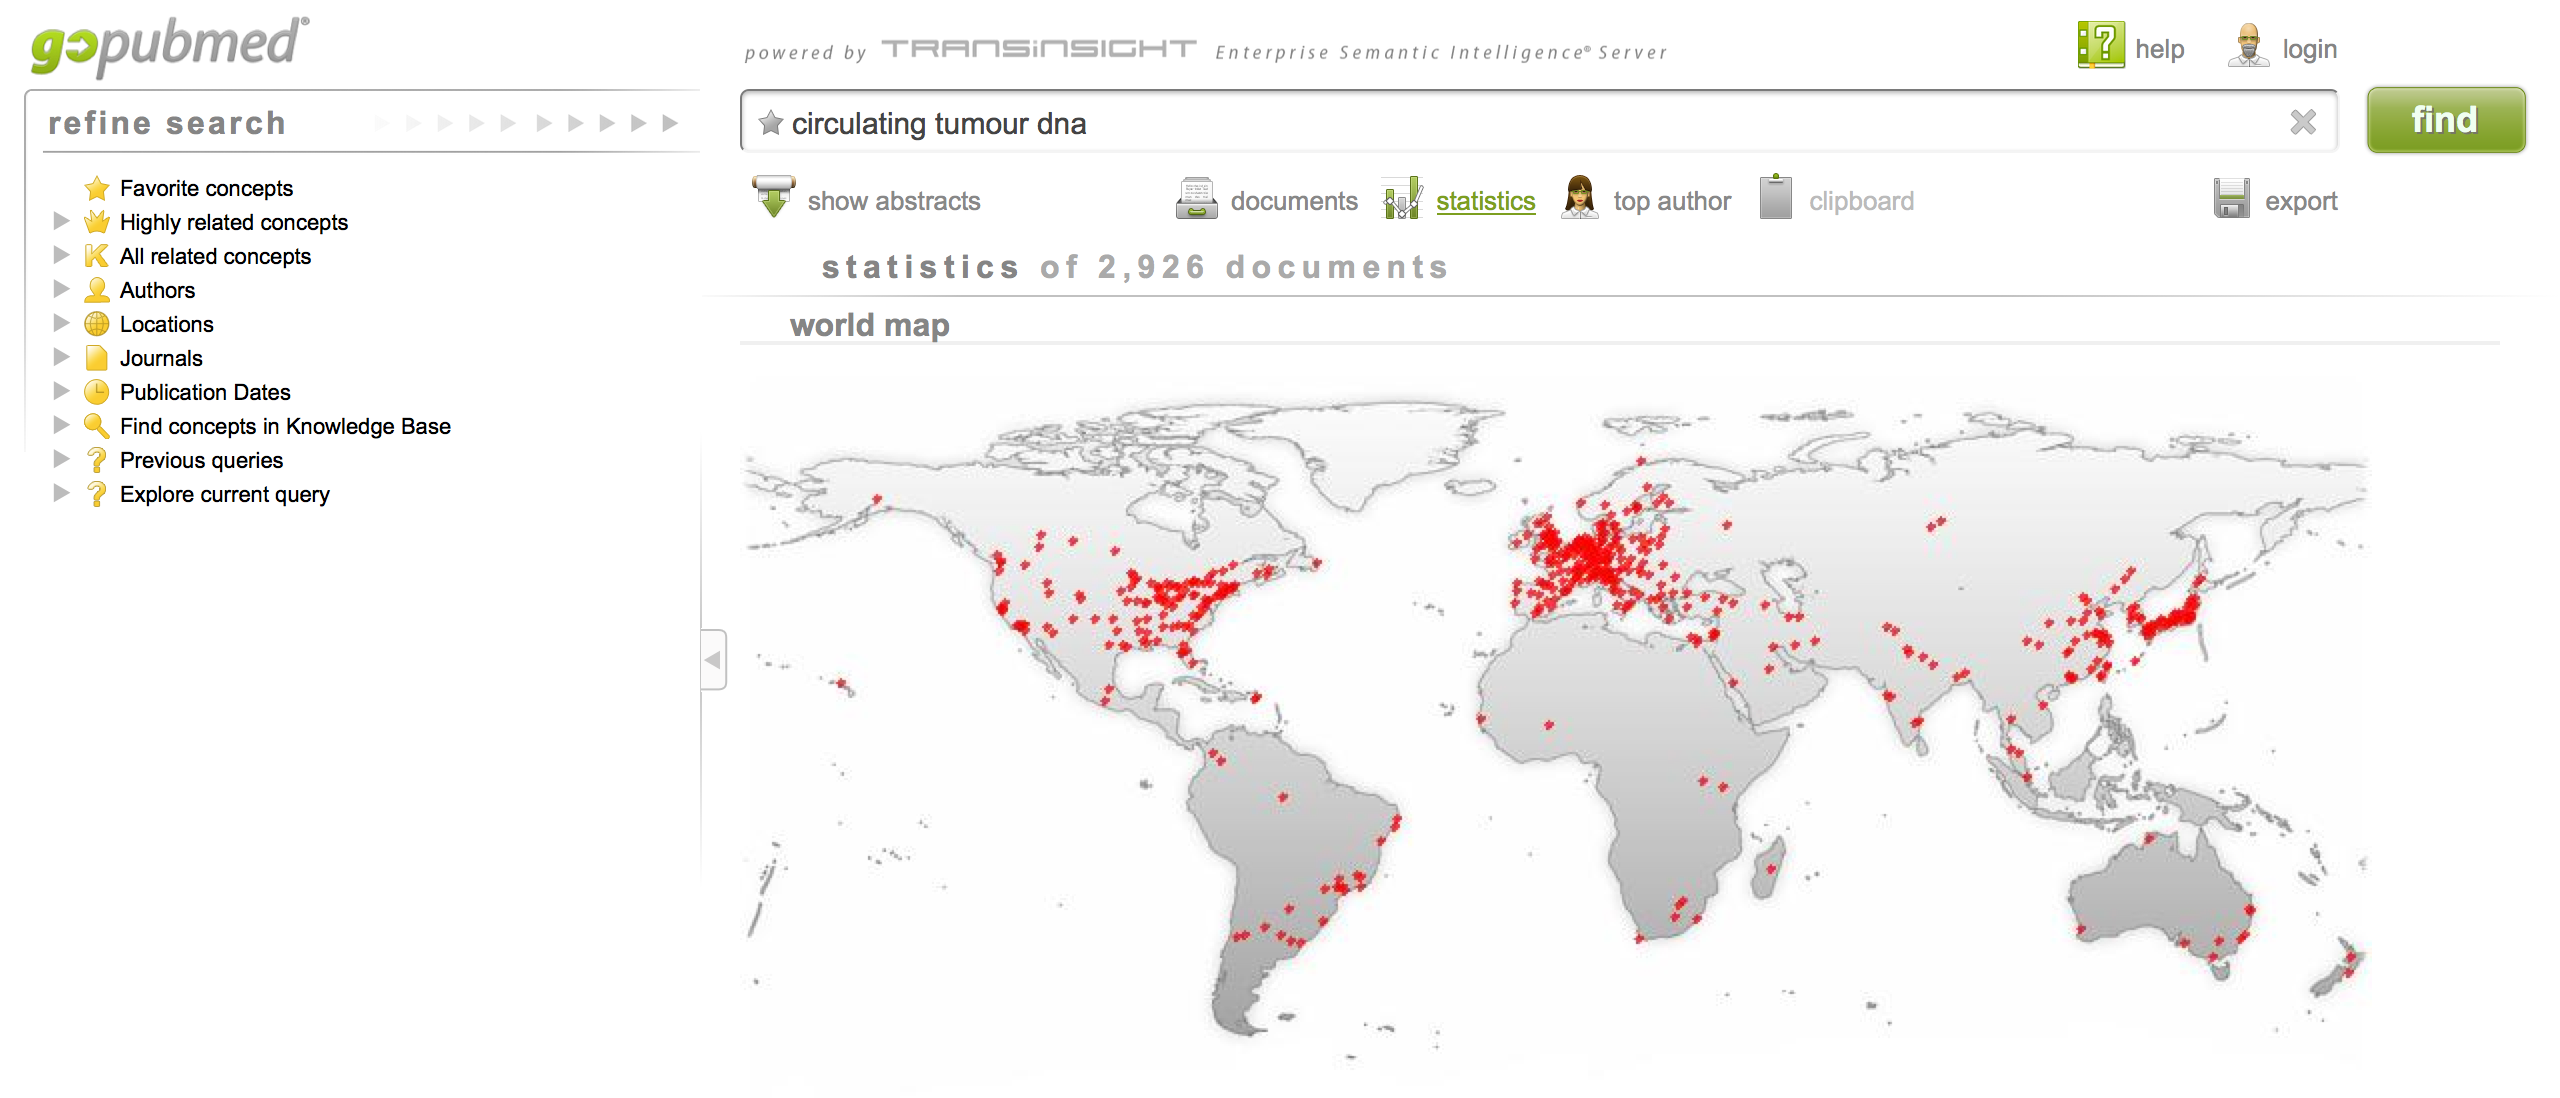
\includegraphics[width=\textwidth]{../lib/images/GPM4}
		\label{fig:GPM4}
		\subcaption{Statistics view: graphics are generated from the documents' associated data. This screenshot demonstrates a generated static JPEG showing the geographical locations of all authors.}
	\end{subfigure} \\
\caption{Web interface of GoPubMed.}
\end{figure}\newpage

\section{Academic Map: Geographical Locations of Institutions and Authors}
The bibliographic search engine Microsoft Academic Search has the potential to be a powerful tool for researchers, as it tackles the pervasive challenge of NED associated with citation data. Several projects were conducted at Microsoft aiming to visualise newly disambiguated data, the most relevant example of which is Academic Map. Browser-based and running on Silverlight, this app represents institutions as coloured circles on Bing Maps (Fig.2). Each circle represents an institution at small scales, but merge together when the user zooms out. This prevents overcrowding of datapoints, easing visual interpretation. There is a search bar available for typing in institution and author names, however due to the inability of the app to locate University College London, there appear to be problems with resolving certain institutions, potentially those that are present at multiple sites. The information available is very high-level, in that interaction with authors or institutions triggers navigation away from the service to new page. For this reason, the utility of Academic Map is somewhat limited without the integration of MAS pages. \\

\begin{figure}[ht]
	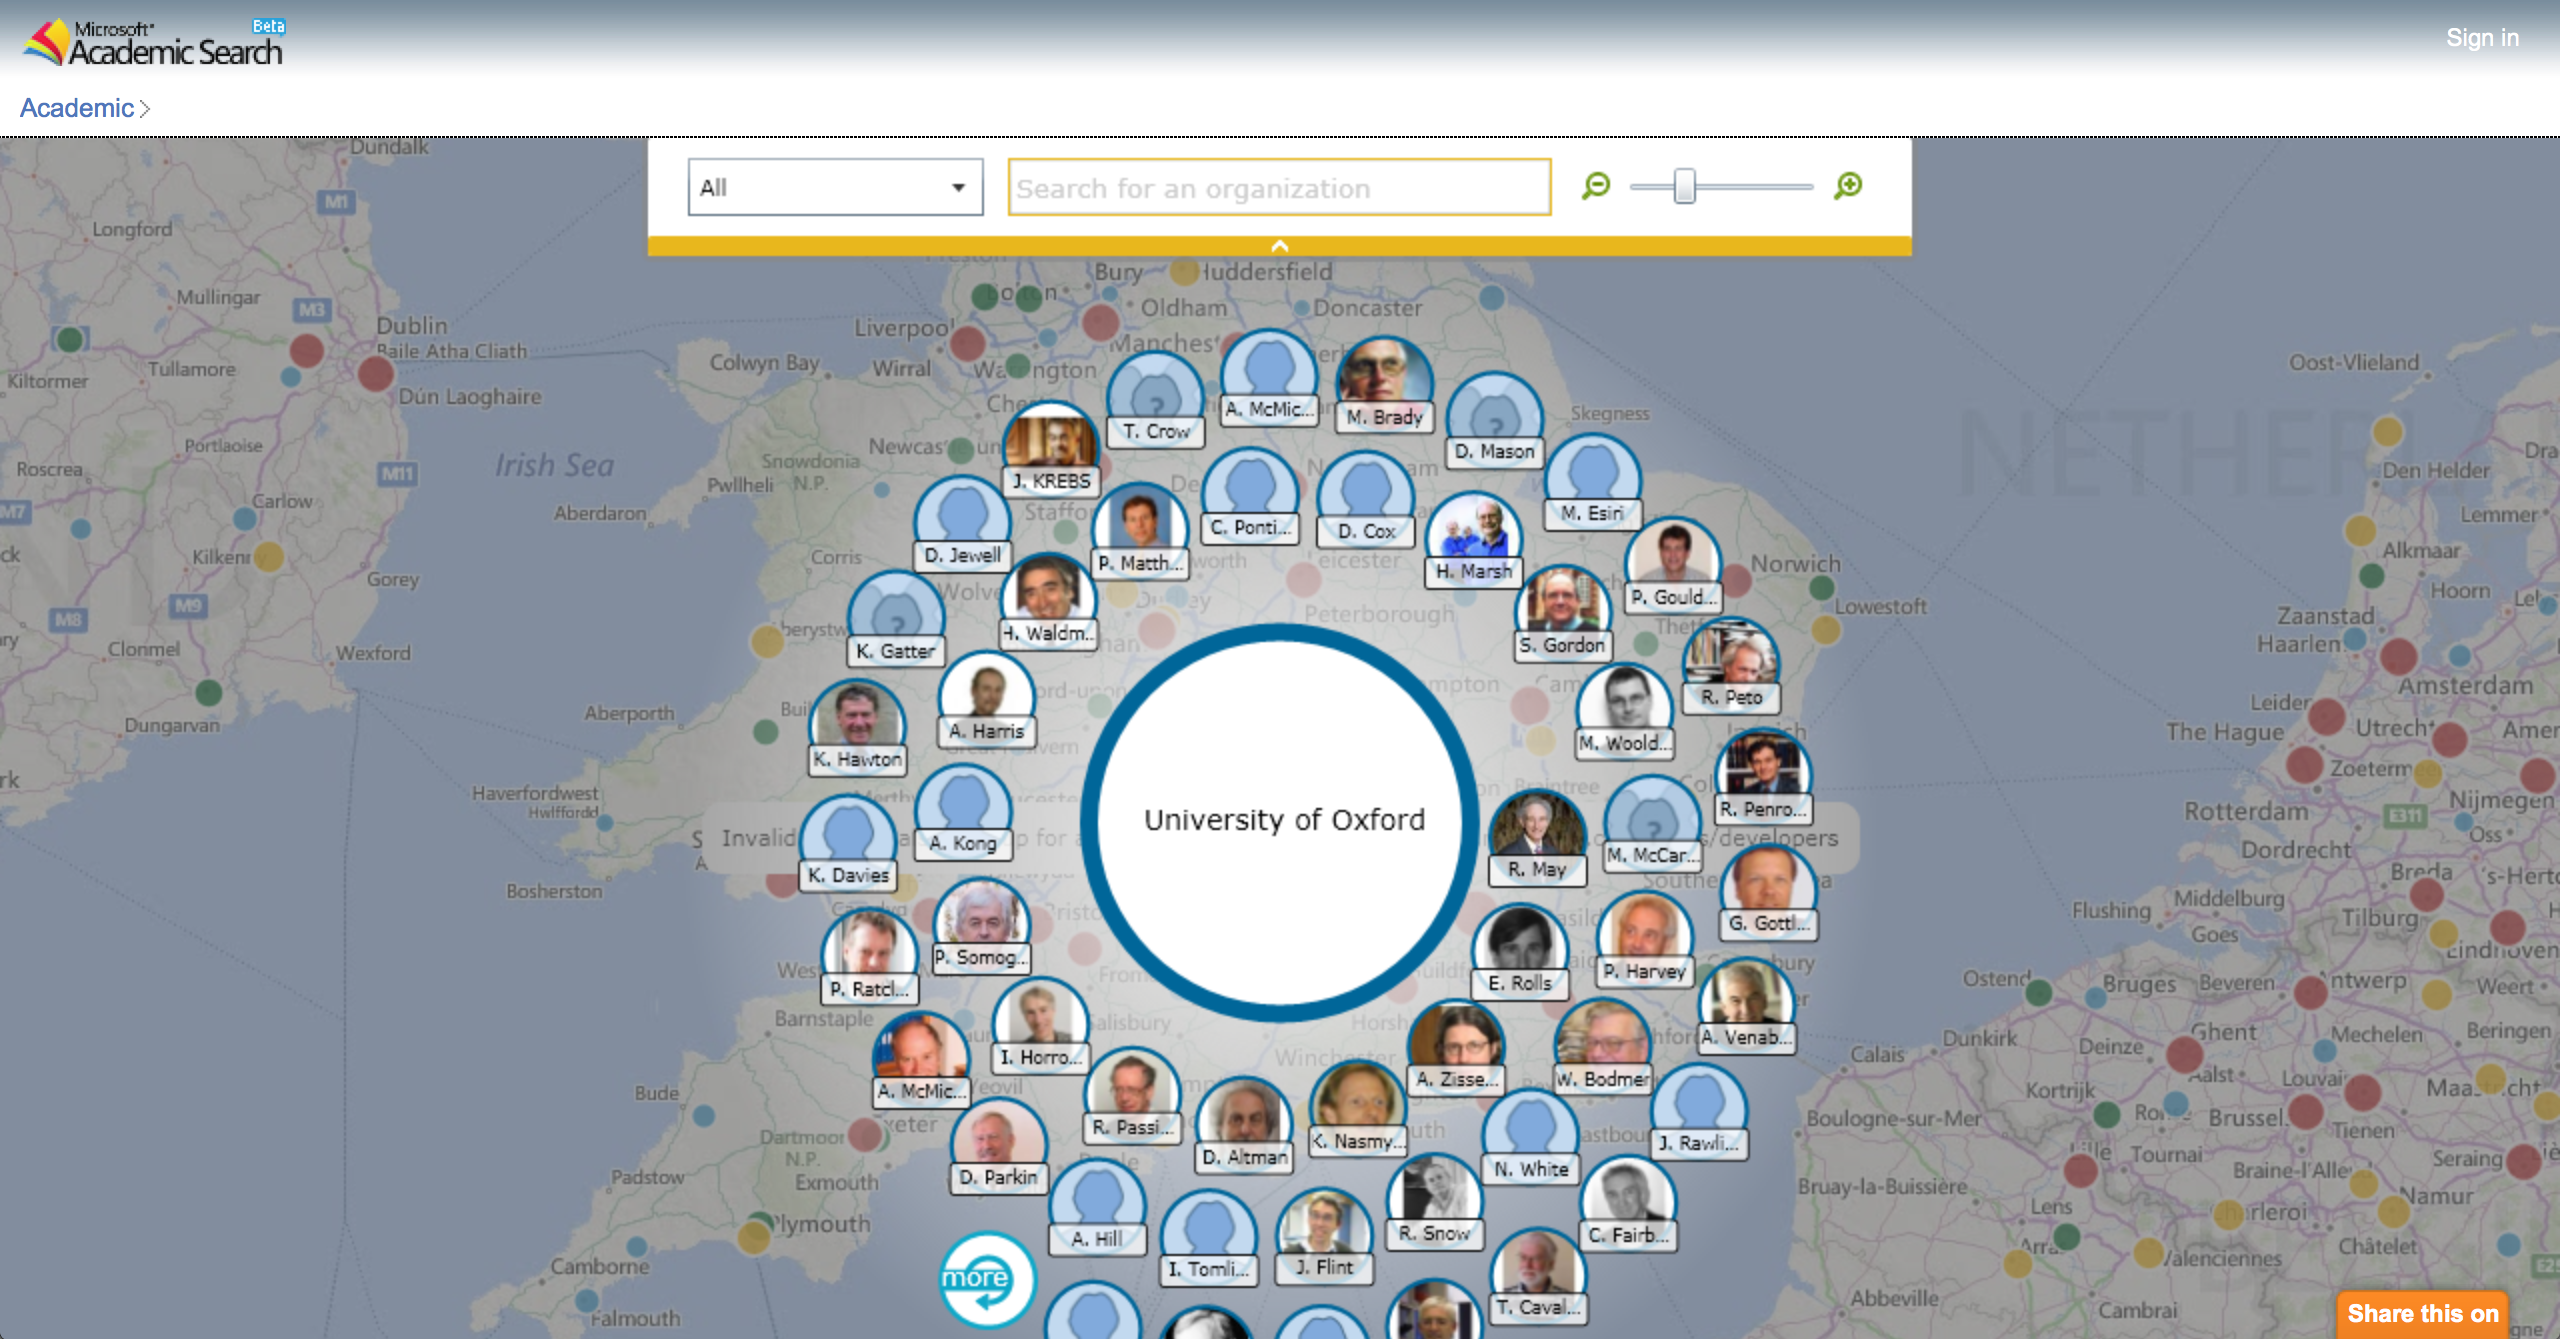
\includegraphics[width=\textwidth]{../lib/images/AM}
	\label{fig:AM}
\caption{A screenshot of Academic Map after clicking on an institution (Oxford University). Each node represents an academic that has published at that location, and selecting this will open the author page on MAS.}
\end{figure}

\section{VOSviewer: Graphical Representation of Networks from Citation Data}
VOSviewer (\url{http://vosviewer.com/}) is a bibliometric network visualisation tool developed by Nees Jan van Eck and Ludo Waltman at Leiden University, designed to enable users to produce clear and informative maps that show relationships within large citation datasets\cite{eck-waltman2}. It is a Java application that is able to handle exported data from PubMed, Web of Science and Scopus, and is free to download and use. Relevant terms are mined from titles and abstracts by extraction and evaluation of noun phrases\cite{eck-waltman1}, allowing creation of network maps based on terms (Fig.3a), organisations or authors (Fig.3b). It is important to note that due to the implementation of bespoke natural language processing of abstracts and titles, this program does not take MeSH or author keywords into consideration. This is an advantage if PubMed is not the sole source of data, or if none are supplied by the authors. For projects that specifically handle data exported from PubMed, it is likely beneficial to use the hierarchical structure of the MeSH vocabulary; doing so aids the separation of synonyms with identical meanings, and allows the developer to specify headings to include or exclude. The clustering algorithms developed for this piece of software go beyond the scope of this project, as the intention is to present the user with a dynamic interface that is transitory by nature. For this reason, accurate representation of the connections between nodes is unnecessary and emphasis will be placed on the speed and ease of use of the data visualisation method.

\begin{figure}
	\begin{subfigure}{1\textwidth}
		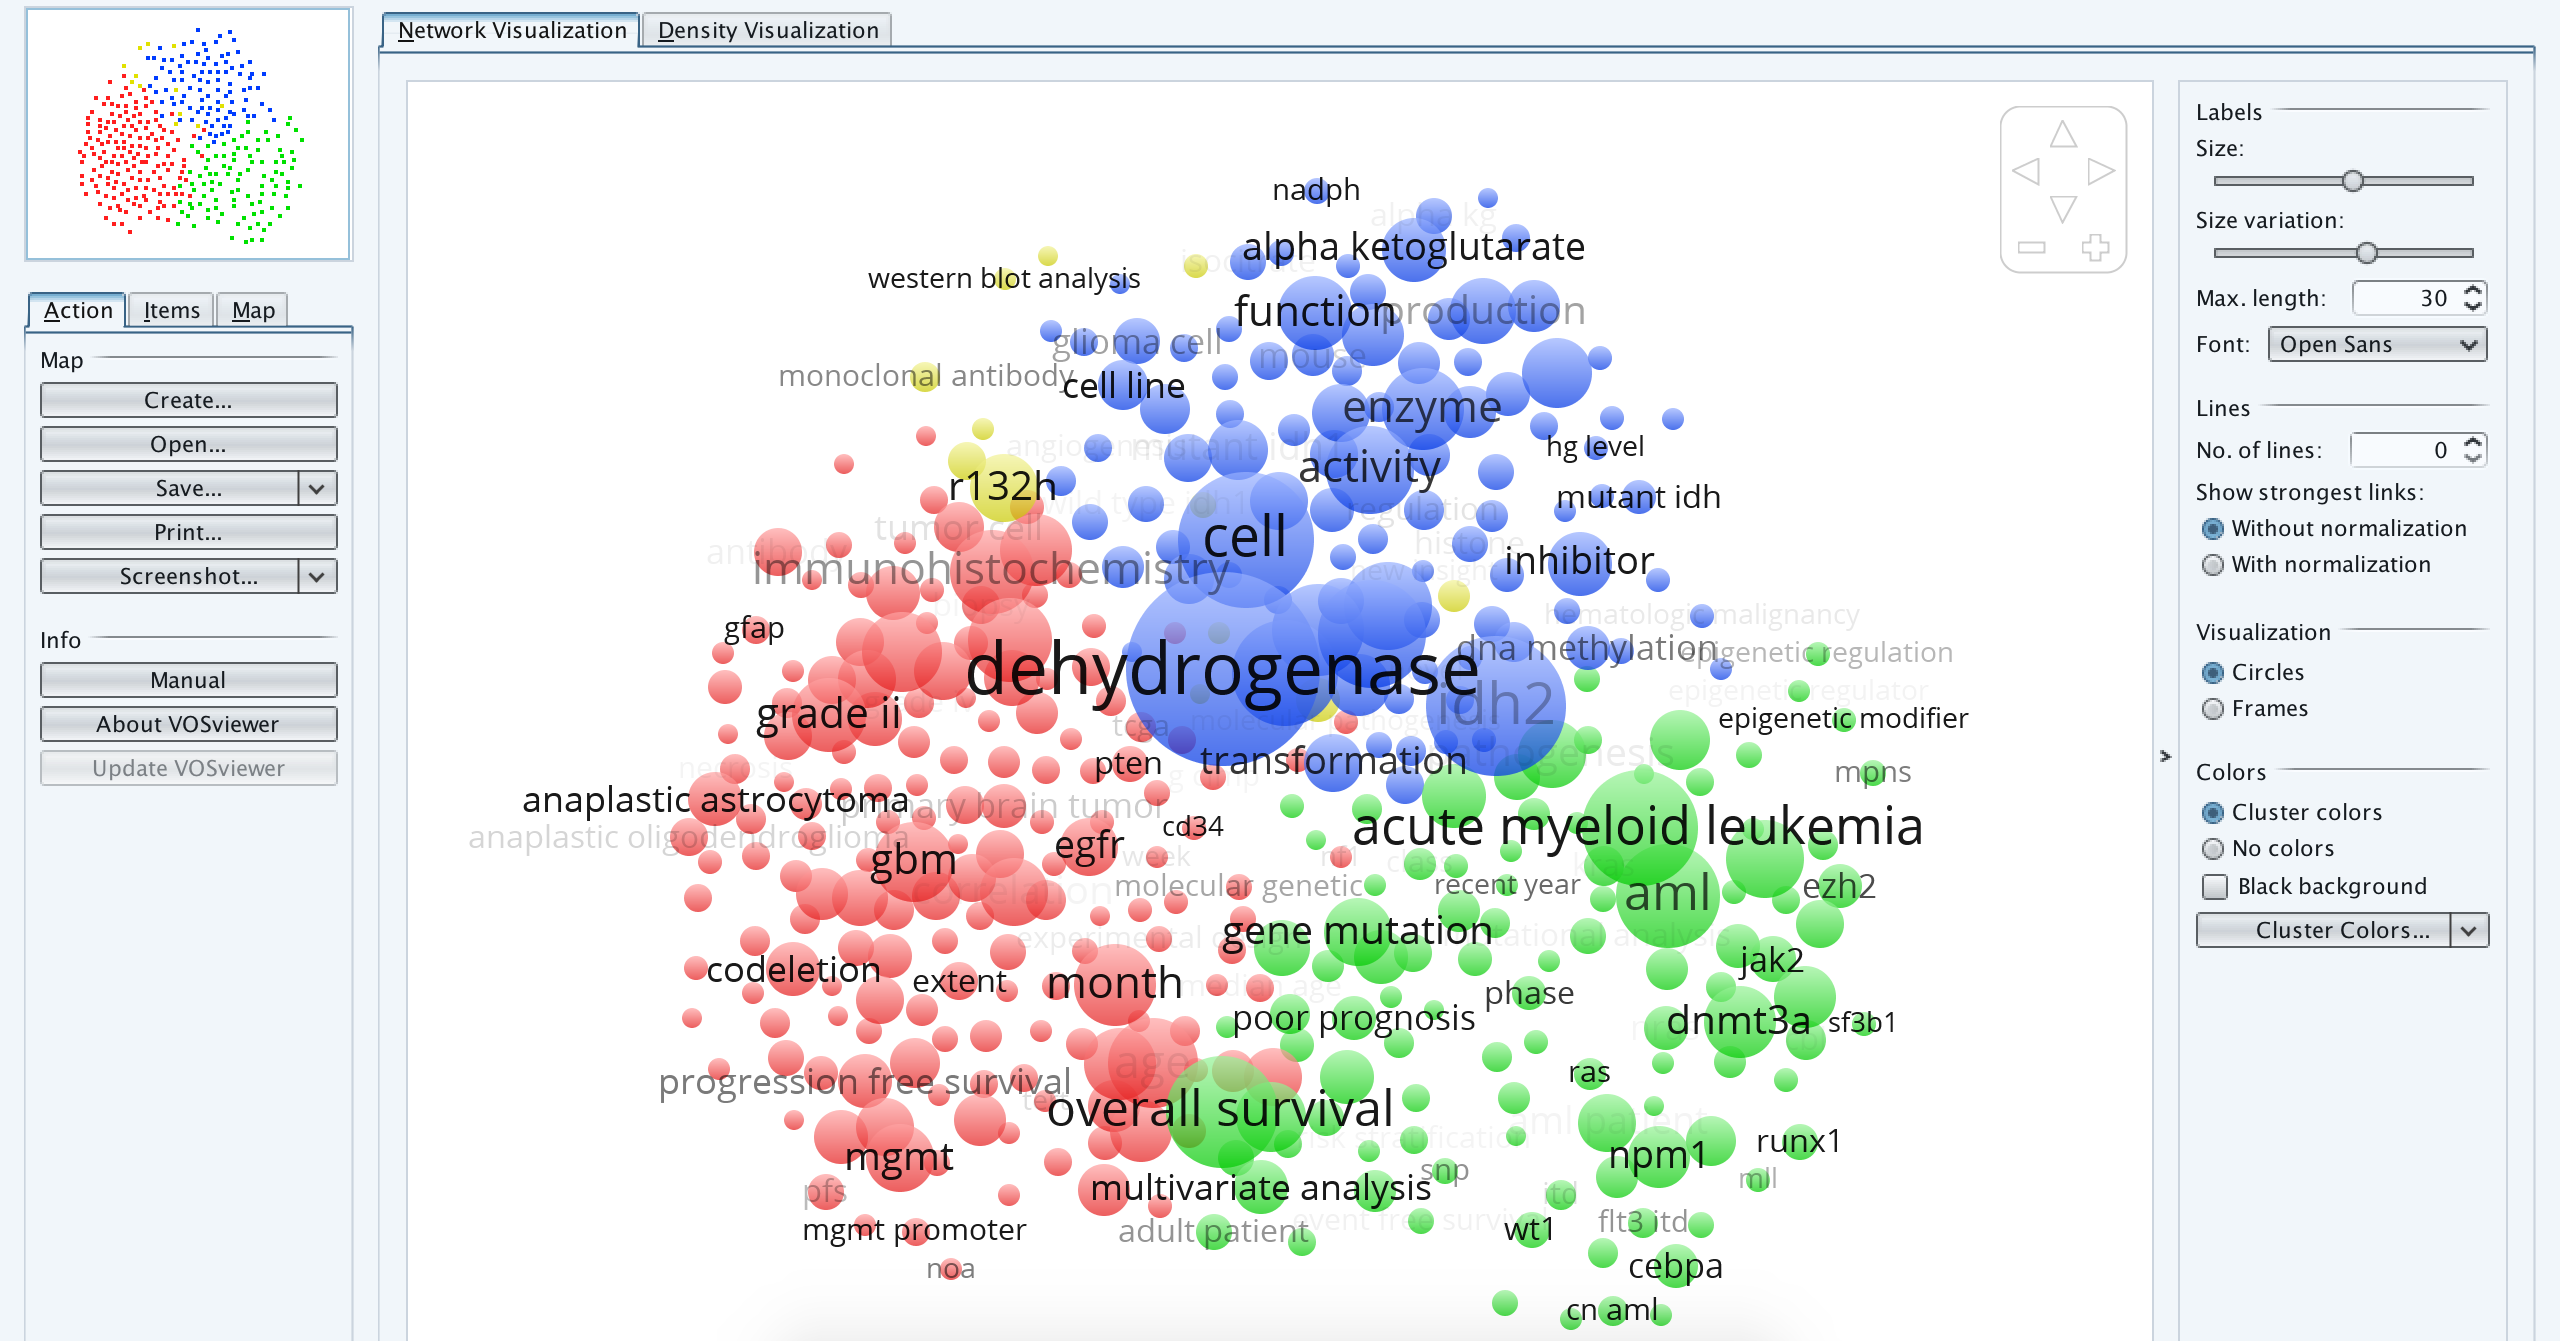
\includegraphics[width=\textwidth]{../lib/images/VV1}
		\label{fig:VV1}
		\subcaption{Terms map generated from a PubMed dataset of 1042 citations with 'IDH1' and 'cancer' searched in all fields\renewcommand{\thefootnote}{\alph{footnote}}\footnotemark[1]. Nodes are coloured by term type, sized by occurrence and clustered by co-occurrence. These features are customisable as can be seen from the panes on each side.}
	\end{subfigure}
	\par\bigskip
	\begin{subfigure}{1\textwidth}
		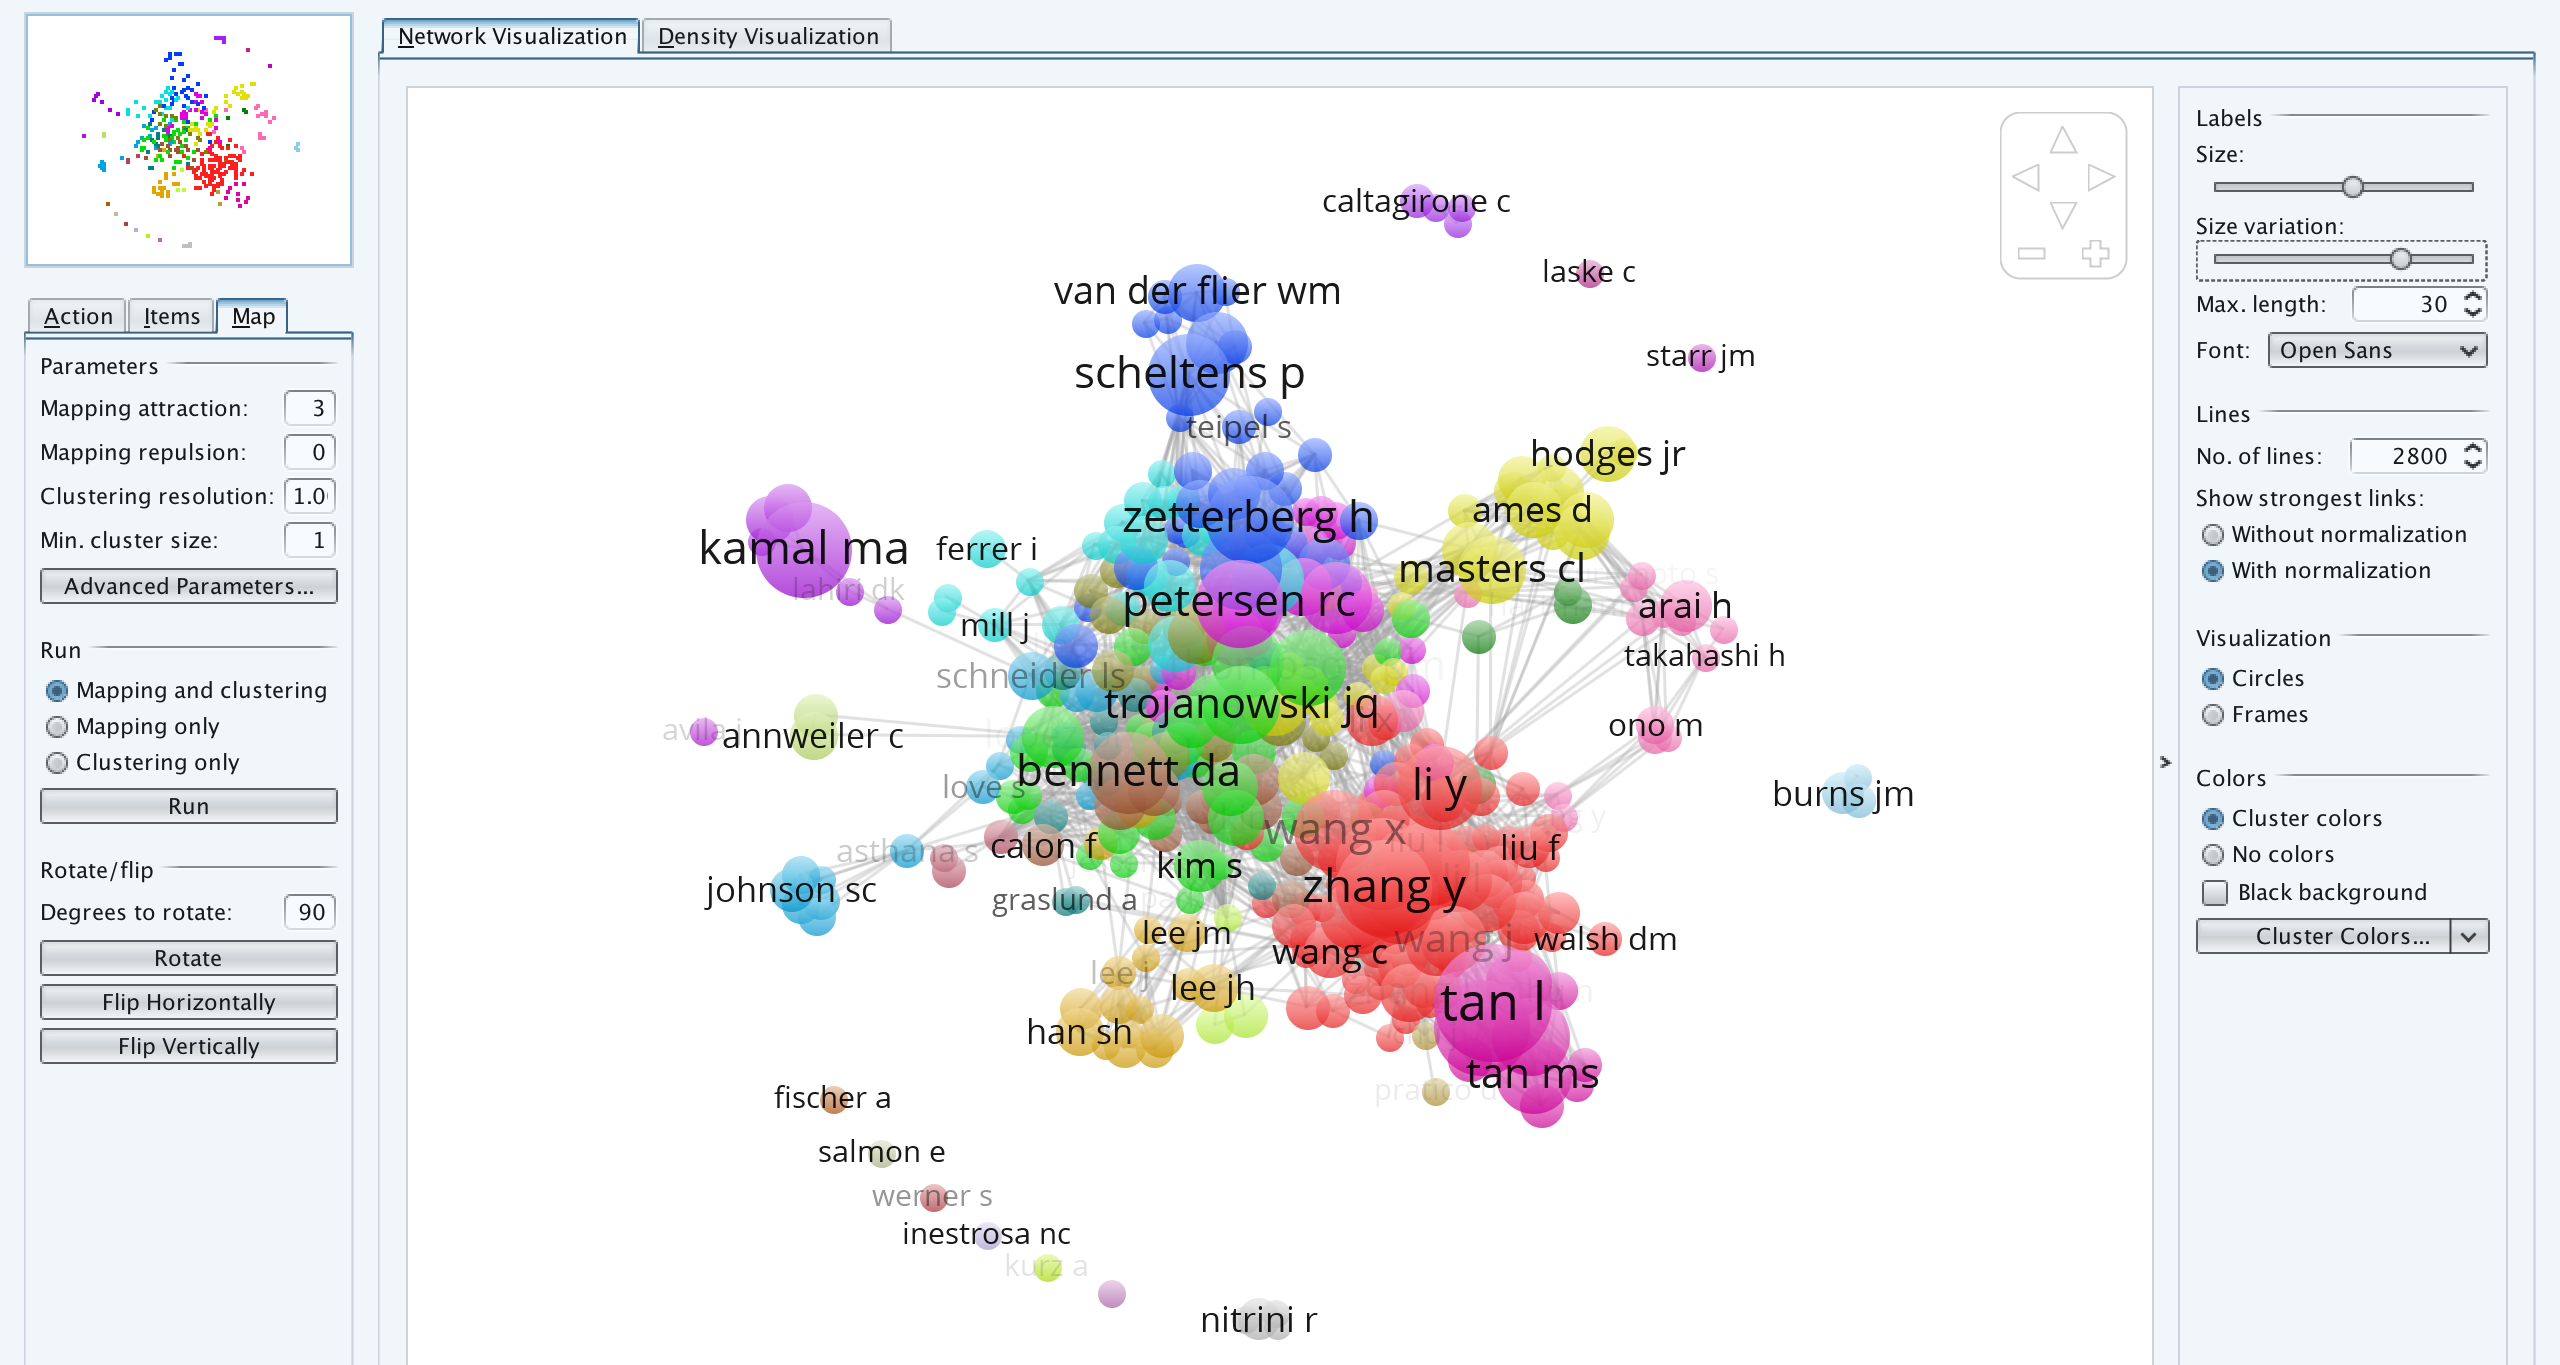
\includegraphics[width=\textwidth]{../lib/images/VV2}
		\label{fig:VV2}
		\subcaption{Authors map generated from a PubMed dataset of 2895 citations with 'Alzheimer's Disease' in the MeSH terms, published since January 1st 2014\footnote{Query ran 08/04/15.}. Node colourings, clusters and lines are determined by co-citations.}
	\end{subfigure} 
\caption{Network maps created using VOSviewer.}
\end{figure}

\section{Discussion}
These three technologies combined solve many of the problems that this project aims to address, namely disambiguation of institutions, graphical representation of results, and network visualisation of scientific terms. GoPubMed is an interesting example of extending the PubMed experience by both directly processing search results and presenting additional methods for filtering and selecting datasets. The key differences between GoPubMed and the proposed project lie in the user interface. I propose a simplified set of filter categories, based on the aforementioned research carried out on PubMed usage\cite{dogan}, and a visual representation of results. The latter will be influenced by the analysis of Academic Map and VOSviewer, which have informed the project in terms of interactivity of geographical maps and presentation of interconnected data, respectively. 

\end{document}